\chapter{Background}     

\section{Introduction}
Web applications has in the last few years seen a dramatic change in both behavior and magnitude. They have grown from being a set simple consistent web pages into highly dynamic, and interactive applications with rich user interfaces. Previously, interactive behavior in web sites were usually performed by Java applets and Flash applications \cite{spa} that could run inside the browser. But as JavaScript engines and web browsers has become significantly powerful, such behavior is increasingly being implemented exclusively with JavaScript.\cite{spa} Together with this shift towards highly interactive web applications, the user behavior is at the same time increasingly becoming more social. Users makes up the main data content of web applications by socially interacting with each other and adding content to the pages. 

This chapter outlines recent trends in applications that can be found on the Internet; commonly named as Web 2.0.\cite{web2.0} We will look at the technologies that enables applications to run on the Internet, and more specifically, the software architectures and technologies that are commonly used for developing traditional Web 2.0 applications. 

The chapter begins with a short history of the world wide web, then a discussion of how the web has changed from being simple and static web documents, into dynamic Web 2.0 applications.  Then, we present an overview of the key attributes and common user behavior that is found in modern web applications. Finally an overview of the software architectures and technologies that are commonly used to implement such applications will be given. This background material will be the foundation of the study that has been done in this thesis.


\section{From Web Sites to Web Apps}

\subsection{History of The World Wide Web}
The World Wide Web (www) was first introduced by Sir Tim Berners Lee at the CERN research laboratory in 1989 \cite{firstweb}. He laid out a proposal for a way of managing information on the Internet through hypertext, which is the familiar point-and-click navigation system to browse web pages by following links. At this time, Tim Berners Lee had developed all the tools necessary to browse the Internet. This included the HyperText Transfer Protocol (HTTP), which is the protocol used to request and receive web pages. The HyperText Markup Language (HTML), which is a markup language that describes how information is to be structured on a given web page. The first web server that could deliver web pages, and he built a combined web browser and editor that was able to interpret and display HTML pages. By 1993, CERN declared that the World Wide Web would be open for use by anyone \cite{historyWeb}. This same year, the first widely known graphical browser was released under the name Mosaic \cite{mosaic}, which would later become the popular Netscape browser. Later in 1995, Microsoft would release their compelling browser Internet Explorer, leading to the first "browser wars" where each one would try and add more features to the Web. \footnote{The technology behind the first version of Microsoft's browser was also based on Mosaic. Microsoft was became licensed to use Mosaic in 1995,\cite{iemosaic} which lead to Internet Explorer 1.0.} Unfortunately, new features were often prioritized in favor for bug fixes, leading to unstable and unreliable browser behavior. Example outcomes were the Microsoft's Cascading Style Sheet (CSS)\cite{css}, which is a language that describes how the HTML elements should appear in the browser. And also, Netscape's JavaScript \cite{jsHistory} was developed to add dynamic behavior that could run in the browser. Microsoft created a replicated version of JavaScript, which they named JScript.\cite{jscript}

\subsection{The Early Days}
In the mid 90's, web sites were mostly \textbf{static}, meaning that the documents received from a web server were exactly the same each time it was requested. This was only natural, as the majority of web sites were pre-generated HTML pages with lots of static content, e.g a company's, or a person's home page. Later, however the need for user input became apparent as applications like e-commerce would require two-way communication. User input was not part of the first version of HTML (1.0), which led to the development of HTML 2.0. This standard included \textbf{web forms}, which allowed users to enter data and make choices that was sent to the web server. The development of web sites grew into becoming \textbf{dynamic} web pages. This means that the server responds with different content depending on the input received in HTTP requests. To enable this, there has to be a program running in the web browser, that can evaluate the HTTP request, and generate a proper HTML page depending on the request itself, and the application's state. This is called \textit{server-side dynamic page generation} \cite[p.691]{tanumbaum}. Another common scenario is \textit{client-side dynamic web page generation}, in which a program is sent to the browser, and executed inside the browser. Examples are JavaScript programs that can achieve dynamic behavior without consulting the server, and applets, which are programs that are compiled to machine code on the client's machine and executed inside the browser. Since applets are compiled to machine code, they execute faster then JavaScript, and therefore, such technologies has for long been favored for implementing performance demanding behavior in the browser. Examples are Java applets, Microsoft's ActiveX,\cite{activex} and Adobe's Flash.\cite{flash} Java applets are executed on the Java Virtual Machine, which is a cross-platform solution and hence portable to "all" execution environments. Therefore Java applets have been a highly popular way of achieving interactive and dynamic behavior in browsers. Examples include browser games, movies and 3D modeling applications. 

\subsubsection{The Problem with Client-side Technologies}
Java applets and Flash had become popular choices for client-side dynamic page generation by the year 2000 \cite[p.2-3]{spa}, and they still exist in many web applications. There are many problems with this approach however. For instance, a plugin is usually required for running such applications inside the browser, and developers need to know an additional programming model, the user interface tend to look different then the rest of the HTML page, and on top of this there has been numerous examples of security violations with the technology itself \cite[p.875-877]{tanumbaum}. Choosing JavaScript primarily would be a preferable solution to client-side interactivity, because it doesn't require an additional programming language or run-time environment considering JavaScript is already supported in all popular browsers. Having one client language is preferable to facilitate a common development model for all web applications. Unfortunately, this technology has also had its issues ever since it was introduced. Partly because of its buggy implementations due to the scurrying development processes in the early browser wars, which has lead to different JavaScript interpreter implementations by the various browser vendors. But also because browsers have not had the ability to execute JavaScript fast enough to enable satisfying dynamic behavior. For this reason, JavaScript has for long been used as an add-on language for HTML to perform simple roll-over effects, input validation and pop-up windows.  

However, a lot of work has been done to provide a standardization of the JavaScript programming language. And lately, browser vendors like Google\cite{google} and Mozilla\cite{mozilla} has improved the engines that executes JavaScript to enable the execution of performance demanding processing jobs. 

\subsection{Modern Web Applications}
With the increase of performance capacity in modern web browsers, a lot of work has been done to standardize the development of the Web applications, such that cross-platform applications can easer be built and be supported in all browsers. Examples include the work on the newest version of HTML (HTML5). This dramatically simplifies the development of dynamic and interactive client-side behavior and media incorporation without the need for additional plugins. Also, the work on improving the JavaScript language itself has made it the assembly language of the web, and is now one of the most popular programming languages in the world \cite{jsPopularity}. With this trend towards client-side development, the web has seen an expanding growth in web sites with rich user interfaces and lots of interactive behavior. The technologies has enabled developers to build web sites that looks more like desktop applications with a responsive user interface. Such applications are often referred to as \textbf{"Web apps"}, where the browser is the main execution platform. We will continue using the term \textit{Web app} in this thesis, to refer to interactive and responsive Web applications with rich user interfaces.

\subsubsection{The Social Web}
In addition to interactivity and responsive behavior, there is another trend that is a increasingly becoming a key factor in modern Web apps; namely social interactions. Many modern Web apps base the information content that makes up the site on what the users adds to the page. Usually this includes users posting blog posts, comments, images and other sorts of data information. And in addition, the users connect to each other in a "social network". Popular "pure" social network applications are Facebook,\cite{face} Twitter,\cite{twitter} Pinterest \cite{pinterest} and many others. In addition to Web apps that serves primarily to connect users, many other types of applications like e-commerce and e-learning adds social networking ability to their web sites as a way to attract more users, and to get better user-data to improve business value. Examples include Airbnb,\cite{airbnb} Amazon,\cite{amazon} (both e-commerce) and Coursera (e-learning). \cite{coursera} 

This behavioral trend has become highly popular, especially considering the users accesses the applications not only on their desktop or laptop machines, but also on smart phones, tablets, TVs, game console etc. Many people accesses their favorite social networking sites up to multiple times a day. This results in huge numbers of simultaneous users accessing their social Web apps, leading to high network traffic on the servers that hosts these apps. The scalability requirements are massive, enforcing software engineers to design for highly scalable, and efficient backend solutions.

Applications that incorporates social networking features and lets users add content naturally leads to large quantities of persisted data. This has led to the term "big data" \cite{bigdata} which describes such extremely large data quantity scenarios that requires highly efficient and extensible persistency systems. Many new database management systems has lately been introduced to the web marked, since the need to persist large data quantities has increased massively the last few years. Such technologies often have in common that they don't follow the traditional relational database structure (I.e SQL-based), but adopts other less structural approaches. Such databases are commonly being referred to as NoSQL.\cite{nosql} The reason they don't adhere to the traditional relational structure like SQL is that this technology has showed not be fairly suited to be distributed over many database servers, e.g in cloud environments. \cite{cloudmanagement} This is a severe problem, because the ability to scale over many machines is not only feasible for load balancing, but an absolute requirement when extremely large amounts of data must be persisted. Most noSQL databases on the other hand, has showed its ability to scale very well over multiple servers, making it a good choice for persistence solutions, especially when web apps are deployed in the cloud. 

A final note with the Web applications just described is that they often offer their services to external third party clients through, what's commonly called their ``public API''. This means that other external applications, (e.g some other Web app) might use functionality that the app is offering publicly as a service, and incorporate this functionality into their own app. This is called a service-oriented architecture.\cite{soa} An example is that some Web app A uses geographic data that they fetch from the public API offered by Google Maps.\cite{googlemaps} 

The applications described in this section are commonly referred to as Web 2.0. \cite{web2.0} The term has a widespread meaning and a lack of consensus on its true definition. However, in this thesis we will use the term Web 2.0 as Web apps that incorporates social networking and public API offerings.

\section{Web Technologies}
Having looked at how the Web started, and given an overview of common attributes and features for Web 2.0 apps, we will now focus on the technologies that hosts these applications. In this section we will discuss the main technologies that are used to build and host modern Web 2.0 apps. First, an introduction will be given on the client-side technologies that executes the Web apps, then we discuss some common architectures and principles for designing these Web apps.

\subsection{Web and Application Servers}
Also called HTTP server, is a program running on a dedicated server machine, that hosts web content to client users. The client is usually a web browser, but it could also be a web crawler, who often intends to gather information on web pages searching purposes. The web server manages  HTTP communication with the client users, and serves static content like images, videos, or stylesheet files. Examples of commonly used web servers are Apache Web Server,\cite{apache} and Microsoft Internet Information Server.\cite{iis} The web server is responsible for delegating requests for dynamic content to an \textbf{application server}. The application server hosts the web application itself, also called the backend, \footnote{The application's \textbf{backend} is the application-code that runs on the server, in conjunction to the application's \textbf{front-end} which concerns the code that runs in the browser.}, and hides the low level details of HTTP requests, typically by wrapping HTTP-header info into separate programming language variables. The application server can route specific URL requests to appropriate handlers in the web application.  Application servers usually supports one or more \textbf{web application frameworks}, which simplifies the development of a web application in a specific programming language. Examples are SpringMVC for Java \cite{expertsOneToOne}, Ruby on Rails for Ruby,\cite{rails} and Django for Python.\cite{django} 

\subsection{The Web Browser}
Browsers are software applications that requests and displays content on the Internet. The information is usually expressed in HTML pages, but it can also be other types of data for instance images, script files, PDF files, or videos. The way browsers interprets the data is specified by World Wide Web Consortium (W3C),\cite{w3c} however up until recently, the various browser vendors have usually not completely conformed to the whole specification but instead developed customized solutions. This has caused many compatibility issues for web developers.   

\subsubsection{High-level structure}
The browser's software stack consists of a set of components that each has individual responsibilities, and cooperates with the work of fetching and displaying web resources. The main components are listed below :
\begin {enumerate}
\item User interface
\item Browser engine
\item Rendering engine
\item Networking
\item JavaScript interpreter
\item UI backend
\item Data persistence
\end{enumerate} 

The rendering engine is a very important part in the process of displaying a resource. Its responsibility is to get the document from the network layer (usually 8 bits at a time), render the document and finally paint the result on the display. The process of rendering the document is showed in figure \vref{fig:render}. Note that this process is iterative and will happen repetitively until the whole HTML page with all its external resources are completely processed. The rendering engine's lifetime is \textbf{single-threaded} and runs in an infinite loop that listens to events. An event might be to calculate a new position of an element, perform painting on new or modified HTML elements or handle a mouse click. However, if multiple external resources are to be fetched at the same time, the browser can, and often will create multiple HTTP connections that will run in parallel to efficiently load content that needs to be contained in the main HTML document. 

\begin{figure}
\begin{center}
\fbox{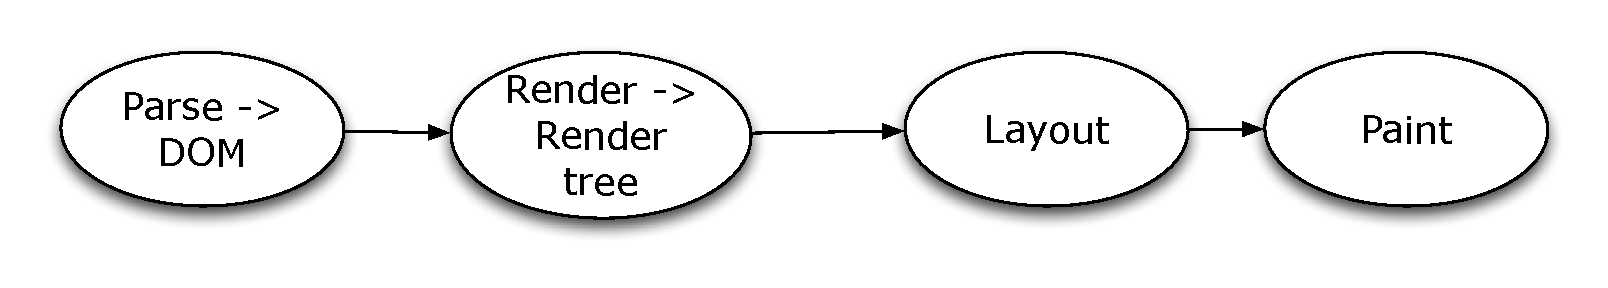
\includegraphics[width=11cm]
{rendering.eps}}
% Kommandoen \fbox tegner en ramme.
\end{center}
\caption{The rendering engine's responsibility}\label{fig:render}
\end{figure}

WebKit\cite{webkit} and Gecko\cite{gecko} are two popular rendering engines that implements the rendering process in the figure, however they do differentiate slightly in their internal behavior. WebKit is the engine that runs Chrome and Safari, while Gecko runs Firefox. In this section we  limit the discussion to concern only these platforms, as they are built upon open source solutions and hence have available technical descriptions. The text that follows describes the process of rendering a complete HTML page. This usually happens when the client-browser requests a URL for an HTML page and the browser "refreshes" the page with the new content.

\paragraph{Parsing} 
The rendering of an HTML page starts when the networking layer is instructed to fetch a URL, say \textit{www.google.com}. As the HTML page is fetched, the browser will immediately start fetching all external \textbf{links} that are contained inside the HTML page. This could be links to stylesheet pages, JavaScript pages, images, videos, etc. As soon as the initial HTML page is received in the networking layer, the rendering engine will start requesting chunks of data. Then it will start and \textbf{parse} the HTML and stylesheet documents. An important feature of the HTML document's structure is that all the markup elements (tags) are nested in a hierarchical structure. Hence, when the HTML document is parsed, its tags are laid out in a tree structure, and if an error is found in the page's structure or syntax, an error is thrown. Note however that the HTML parser is "forgiving" in that it will fix errors found in the HTML document.

Whenever the parser hits a script tag, it will first fetch the script if it is referencing an external file. Then, it will execute the script immediately. Unless the tag is marked "deferred" in with case the handling of the script will be postponed until the HTML parsing is done, the parser has to wait until the script is both fetched and executed. This is because the script might try to manipulate the DOM tree. To improve performance by avoiding the HTML parser to block while scripts are loaded, scripts can also be marked as "async" in which case the modern browser will to generate a separate thread that fetches (if needed) and parses the script asynchronously in a separate thread, while the main parser thread can continue parse HTML. 
 
 The tree that is generated is called the \textbf{DOM tree}, where each tree element is named a DOM element. When the whole HTML page is completely parsed, the rendering engine will start executing the scripts that are marked   "deferred". When these scripts are finished executing, the browser will generate a \textbf{DOMContentLoaded} event. Finally, if there are any depending scripts that were marked "async" that are still being fetched or executed, and when all external resources are fetched, the window's \textbf{load event} is generated. 

\paragraph{Rendering}
While the DOM tree is being populated, the rendering engine will also start generating the \textbf{Render tree}. This is another tree that is a visual representation of the DOM tree, and in effect decides the style and order of how the DOM elements should be laid out. Every element in the Render tree has a reference to its DOM node, a style, and in addition they know how to layout and paint itself and its children. In effect each render element represents a visual \textbf{rectangle} on the screen. However, it is not necessarily a one-to-one mapping between a DOM element and its render element, because some DOM elements may need multiple rectangles on the screen, and hence have multiple render elements attached to it. The rendering tree is generated from all the styling elements contained in stylesheet documents, styling information in the HTML document, and default styles provided by the browser. While attaching render elements to DOM elements; if the stylesheet is not fully loaded yet, it will save a  "holder", so it can continue later.

\paragraph{Layout}
In the layout process, each render element is given coordinate instructions for where on the screen it will be placed, and the sizes it will be given. The calculation is performed recursively from the root HTML node to the bottom. Also, the layout process can be \textit{global} in which the entire rendering tree performs layout calculation, or \textit{incremental} in which case it uses a dirty bit system; each time a new render element is added or modified it is marked dirty. When an incremental layout process happens it will calculate only the render elements that are marked dirty.

\paragraph{Painting}
The painting process does the actual work of painting the elements on the screen. It does so by iterating through the rendering tree and paints each component. Like the layout calculation, painting can also be done globally on the whole rendering tree, or incrementally. In the latter case, whenever a render element is changed in a way that does not affect the entire tree, the renderer will cause the OS to recognize the changed renderer and hence trigger a \textbf{paint event}.
 
\subsection{JavaScript}
JavaScript is an interpreted programming language primarily built for manipulating web pages. The language was developed at Netscape in 1995, during the time when Netscape and Microsoft were battling for the majority of browser users. The language itself was built in only 10 days, by Brendan Eich.\cite{jsin10days} He had instructions to develop a language that would look like Sun's Java, only simpler, interpreted and easy to integrate into web pages, so that it would appeal to non-professional developers. The reason was that at the time, Netscape was built with Java, and the browser-server model was considered a distributed application environment supporting cross-platform development. The only problem was that HTML wasn't sufficient to support complex programming operations, and Java was a rich, and comprehensive language aimed for professional developers \cite{jsin10days}. Hence the need for a hybrid solution. Eich designed the language to follow much of the syntax from the C programming language, only simpler and a much more dynamic memory management system. At the time, a web page's lifetime would usually last from a few seconds to a couple of minutes, so therefore the language had only a simplified concurrency model and memory management \cite{jsin10days}.

Despite a considerable amount of buggy features in the language and some compatibility issues between the different browsers, JavaScript quickly became a highly popular language for the web. Developers easily create interactive behavior like changing color on a button when a mouse hovers over it, give the user feedback if the input in a textfield is wrong etc. Much of its success was because of its simplicity; there was a low barrier to add JavaScript behavior into web sites. Because there is no compilation process, and no "start function", only independent functions that can easily be written and ``tossed'' around in the document, unprofessional developers could quickly implement exciting and dynamic features \cite{jsHowGotHere}. On the other hand, for this reason, many professional developers would consider the language of being strictly for amateurs and not suitable for professional developers \cite{UnderstoodJs}.  Its strength, however, was clearly for small sized applications, as browsers at the time were not able to execute large-scale JavaScript code. Also, considering that the JavaScript language at the time was very simple and limited, the development of large-scale JavaScript Web apps was simply not feasible. 
 
In an effort to improve the language features of JavaScript, and its browser incompatibilities, a standardization process of JavaScript was given to the European Computer Manufacturers Association (ECMA) in 1996. The language was actually renamed to ECMAScript, although most people still refer to it as JavaScript \cite{jsHist}. Unfortunately, as the standardization was being developed, the browser inconsistencies, especially between Netscape and Internet Explorer continued to grow. Many JavaScript frameworks were built as workarounds to the inconsistencies, but most solutions weren't good enough. This led to alternative solutions for highly interactive and graphical client behavior such as Adobe Flash or Microsoft's Silverlight. \cite{silverlight} 

An important part of JavaScript's history was with the rise of \textbf{Ajax} technologies,\cite{ajax} which gained much attention right around a century after JavaScript was first introduced. Ajax is an API that offers JavaScript functions that makes the browser asynchronously fetch data from the server without having to refresh the current web page. Instead, the requested data would be used to manipulate the web page. This would result in a much more interactive user experience because the browser would neither block while waiting for the request, or re-render and paint the whole DOM tree upon successful complete. Since the introduction to Ajax, JavaScript has increasingly become a highly popular language, and it has brought the attention of professional developers. This has led to successful framework solutions like JQuery\cite{jquery} and Prototype,\cite{prototype} which simplifies the development of complex dynamic behavior and fixes browser incompatibilities, so that the web developer doesn't have to write specialized code for each browser.

The increasing popularity of client-side application development with JavaScript has led to powerful JavaScript engines in modern browsers, making memory management and JavaScript interpretation highly effective. In September 2008, Google built the Chrome browser with its V8 JavaScript engine,\cite{v8} stating that low performance JavaScript implementations are no longer sufficient. Other browser vendors followed along, and today JavaScript performance is more superior than ever. Still, however, there are drawbacks with the language itself. Even though libraries like JQuery and Prototype simplifies the development of interactive and cross-platform web pages, it is easy to end up with a big pile of tangled JavaScript event handlers and unstructured functions. Most of the reason is that the language lacks features like classes, modules and namespaces, which makes it difficult to develop flexible and maintainable large-scale JavaScript applications. However, a lot of work has been done lately to implement quality frameworks that provides comprehensible syntactic sugaring for the language. These frameworks use the nice concepts of the JavaScript language like inheritance and closures to enable a highly flexible and structured development environment. All this has led to a massive amount of large-scale JavaScript web applications where much of the backend code has been moved to the client tier, implemented in pure JavaScript. Good examples are Google's Gmail,\cite{mail} and Maps. \cite{maps} 


\subsection{Client-server Interaction Schemes}
There are multiple ways the browser can communicate with the web server. In this thesis, we mainly adhere to two different ways ways: synchronous client-initiated requests, and asynchronous client/browser-initiated requests. These communication schemes all use HTTP, and are client-pull based. However there are other push-based alternatives like Comet,\cite{comet} or WebSocket,\cite{websocket} where the client and server maintains an open connection, and the server can notifiy the client of changes.

\subsubsection{Synchronous}
In a synchronous HTTP request, the client-browser asks the server for data, in which the browser will wait for the server to respond. The request is normally trigged by the user who writes a URL in the browser and presses enter, or an HTML form that is submitted. This could be a button that is pressed inside an HTML form tag, the enter key is pressed inside a text field that is contained in a form tag, or a link that is clicked on a given page. The server usually responds with a new HTML page that is sent to the browser, in which case the browser would start a complete rendering process to build a new DOM tree, and paint it on the screen. A normal term for this is a page \textit{refresh}, or \textit{reload}.

\subsubsection{Asynchronous}
In asynchronous HTTP requests, the client-browser sends a request to the server and continues to execute without waiting for the server to respond. The request can be initiated by the user, or the browser might trigger the request itself. When the server has completed handling the request, it will send the respond to the browser, which is then notified and will handle the result. Usually in this communication scheme, the result is not a complete HTML page, but rather a more fine-grained data object. In this case the browser would perhaps manipulate the DOM tree to alter the page content in correspondence with the result that came from the server. The browser does not have to reload the page, since the browser's data structures (DOM/rendering trees) does not have to be re-built. The client user is usually unaware of the request, because the browser doesn't block while the communication happens.

The most popular implementation of asynchronous communication with HTTP is Ajax. An Ajax request can be sent to the server, in which case the browser does not have to block while the request is being processed. When the request finishes, and the browser receives the response, the browser will initiate an event, in which the developer would have created an event-handler that parses the result, and performs some action based on the result.  

One potential drawback with Ajax is that not all browsers supports JavaScript. Examples are some smartphone devices or PDA devices. Also, some old browser implementations would not let Ajax requests send the browser to a new \textit{state}. This means that if the user hits the back button after an Ajax request has been performed, the browser would go back to the last full-page reload that was accessed, instead of going back to the page as it was right before the Ajax request. Last, pages that are generated using Ajax are not automatically picked up by web crawlers, because most web crawlers does not access JavaScript code. This means that content generated by Ajax would normally don't show up in public web searches. 

\subsection {Input validation}
Protecting the application from malformed user input is an important aspect of web applications. Not allowing clients to submit illegal input both helps making the users sure they entered the data they intended (humans often makes mistakes), and it protects the application against malformed data that might have bad intentions. Even though the HTML pages might have validation logic built into the page (e.g by JavaScript), there are ways to manipulate the data that is sent with HTTP requests. Examples include SQL-injection attacks \cite{sqlinjection}, or other types of HTML form injections \cite{htmlinjection}, in which the attacker is able to alter the execution of a given form. Therefore, user input should be performed both on the client tier for quick validation feedback, but also on the server, in case the client tries to override the validation in the Html page. 

\subsection{HTTP Sessions}
An HTTP-session is a semi-permanent communication dialogue that exists for two communicating entities (here, the client and the server). A session normally has a time-out value, such that when the time runs out, the session ends. The HTTP protocol is stateless in its nature, because every HTTP request is self-contained, and independent of every other request. Therefore, to be able to maintain state in an application, the client and server has to incorporate a session protocol. The state information itself is data that has to be maintained between multiple pages in the application. Examples are shopping cart information in an e-commerce site, flight booking details, or authentication credentials. Imagine the user having to identify himself for each request he sends to the server. This can be avoided if state information is persisted and being referenced for each request. 

There are a couple of ways to implement sessions. State can be kept and managed on the client, on the server, or both by having state information inside the messages sent between the client and server. As for server generated sessions, an implementation is usually provided by the web application framework that hosts the particular application. In this case, the server generates a session-object that will contain session data. This object can be kept in-memory, in the database or stored in flat files. To identify the session object when a request comes into the server, some web frameworks choose to put a unique id in the HTTP cookie header-field, or if cookies are not supported by the browser, the identifier can be injected inside URLs. The session identifier is then included in every HTTP request the user sends to the server. An example is given in figure \vref{fig:httpsession}. Note that the session object can, and often is used as a cache for data that the given user would access often. That is if the session object lives in the server's memory and not in the database. This avoids having to fetch the same data from the database needless times.

State information can also be maintained inside the messages themselves, that are sent between the client and server. This could be to place the data inside hidden fields in HTML forms, store the data in cookies, or store the data in the URL. However, this approach is not very flexible, as the data has to be manually coded into all the places in the HTML pages where requests are sent to the server, plus that the data size is limited, as is the data format.

A third alternative is to store session state in the client's browser. This works in the same way as the server-side approach, in that a session object is stored in browser memory or some external database managed by the browser. The advantage of this approach is that no session identifier has to be included in the HTTP requests sent to the server, since everything is managed by the client. If the session is to be stored in the browser's memory, the browser has to support HTML5, which provides a programming interface (API) for communicating with an in-memory database in the browser.  

\subsection{Representational State Transfer}
In web applications, each individual HTTP request is handled by a particular function that resides in the application's backend. Modern web applications often follows a design pattern named Representational State Transfer, or simply REST. \cite{armando2012} This pattern states that all HTTP URL's must reference a particular resource on the backend, by using one of the four supported HTTP operations Get, Post, Put, or Delete. This way, every URL offered by the web application are self-contained in that it contains all the necessary information needed to satisfy a request. Resources are identified by a URI, which uniquely identifies a resource, and one of the four HTTP methods that should be performed on the resource. Applications that follows this pattern are named RESTful applications. A common use case for RESTful applications is to offer the self-contained URL's publicly as an API to clients other then just the application's own front-end, like other third party applications that wishes to use the applications REST services. Further, the REST pattern states that each REST request is stateless, hence adhering to the nature of HTTP which is stateless. That means, REST requests should not depend on an ongoing session in order to generate proper results.

\subsection{JSON}
JSON\cite{json} is a text based data format that is based on a subset of the JavaScript programming language. It is easy for both humans to read, and machines to parse, and has a similar syntax to many of the programming languages based on the C family of languages. The data structure fits well as a transmission format in web applications, because it is both simple and light weight, easy to modify and is supported by many programming languages. The format itself is very simple, and the datatypes offered are limited to numbers, strings, arrays, objects (key-value pairs) and booleans. An example of a JSON object representing a guitarist is showed below:
	\begin{lstlisting}
	{
		"username": "Paul Swayer",
		"age":21,
		"country": "Norway"
		"guitars": 
		[
			"Gibson Les Paul",
			"Fender Stratocaster"
		]
	}
	\end{lstlisting}
This object contains two string key-value pairs, one integer value, and one array consisting of two simple string values. Notice how the object itself is made up of key-value pairs. RESTful applications might choose to use JSON as a transmission format. For instance a JSON object can be sent with a PUT request, so that the REST receiver will update the object with the content in the JSON object. Also, in a REST-get request, the receiver can return a JSON object to the client.

The closest alternative to JSON is XML,\cite{xml} which is another transmission format often used on the web, and especially with REST communication. However, its syntax is a bit more verbose, and requires more processing to manage because of its markup tags and syntax rules. On the other hand XML lets one add more restrictions to the data then with JSON.

\subsection{Template Rendering}
In dynamic web pages, when an HTTP request comes in for a particular HTML page, the server has to prepare and populate the HTML page with proper data variables before the completed page is sent back. Normally the server inspects the HTTP request that comes in by looking at the HTTP request headers, the content of the HTTP body, and a session identifier if it's provided. Given the information provided in the request, the server will perform an action, and probably fetch data from the database. This data is to be injected into the HTML page that will be returned to the client.

One way to generate an HTML page that contains the newly generated content, is to generate the HTML directly in code as Strings, and send the result back to the client. However this approach is messy, difficult to maintain, and the developer has to know the programming language that is creating the HTML strings. In other words, not a preferable solution for web designers who only knows HTML. The preferable approach is to use a template system. A template system consists template files (often called views), which are files that consists of HTML with special markup code that refers to and can operate on the data variables in the web application. The operations supported are usually limited to simple loops and conditional expressions, just enough to facilitate the injection of dynamic data without confusing front-end designers. The template system also has a template rendering engine that takes a template file, the data to populate the file, and produces an HTML page. This way, when a client request comes in, the server will generate some data, probably from the database or an in-memory cache, create an object that is filled this data, and send the object together with the proper template page into the template rendering engine. The resulting HTML page is sent back to the client. 

Template rendering can also happen on the client. The process is pretty similar. Rendering is  performed by JavaScript code that ``lives'' inside the HTML page. This is done by adding special syntax in the HTML page that is recognized by a rendering engine, and ignored by the browser. When some HTML page is to be rendered, the JavaScript rendering engine is called with an HTML page and a data object as input, and it would return the same HTML page, but altered with the new content from the data object. Unlike server-side page rendering, there are no special file type for template files. They are just HTML pages with special syntax that is ignored by the browser when the HTML page is rendered. Hence server-side template rendering generates a new file given a template file, while client-side template rendering only modifies an existing HTML file. 

\subsection{Databases}
Storing persistent information is an essential part of web applications. The content that is offered must be able to be saved, retrieved, deleted and modified in an efficient and flexible manner. Databases, and especially relational databases has since the beginning of web application history been the most popular form of storing persistent data.\cite{engineering} Other alternatives have been used like flat-file storage (where the content is stored as plain text or binary data) or XML- or object databases, but ever since relational database management systems arose back in the early 1970s, it has been a highly popular form of data persistence. Much of the reason is that it provides \textbf{durability}, which in the context of data persistency means that once the data is stored, it is guaranteed to exist even if machines holding the data crashes. Also, a reason for the relational databases's popularity is that it stores information in a structured format, which often fits the structured data formats that are manipulated by the web applications. However, as the extent of information being persisted in modern web applications has become incredibly large, other types of database technologies has also entered the marked lately. These are commonly referred to as noSQL databases.

\subsubsection{ACID}
ACID is a popular term in the context of databases. It is a set of properties that guarantees reliability when it comes to transaction management. Database management systems often state that ACID guarantees are provided in their system, in order to promise a reliable database solution. Each property is defined below:
\paragraph{Atomicity} guarantees that either all the commands in a transaction completes, or non no.
\paragraph{Consistency} guarantees that all the data will always be in a consistent state according to pre-defined rules. A transaction brings the system to a new consistent state.
\paragraph{Isolation} guarantees that parallel transaction executions are always processed as if they happen serially, i.e no interference of any two parallel transactions. 
\paragraph{Durability} guarantees that committed transactions are safe, and lasts even during system errors or crashes. 

ACID guarantees are often provided by relational database management systems (RDBMS). However, noSQL databases tend to have a more relaxed relations to the principles, in favor for speed and scaling abilities. 

\subsubsection{CRUD operations}
In web application terminology, one often use the word CRUD to refer to the four essential  database operations; \textit{Create}, \textit{Read}, \textit{Update} and \textit{Delete}. These are operations performed by the web application, on the data that needs to be persisted. When a CRUD operation is executed, it is the application's responsibility to convert the data into a format that fits the database's technology, and vice-versa. This process is called marshaling, or serializing. One example is when the application is to save a new object in the database. In this case, a \textit{Create} operation will be performed where the application will transform the object from whatever programming language syntax the object is currently described in, into a structure that fits the given databases' syntax. The application will send this transformed (marshaled) object to the database, which is now able to parse the object and save it to its storage structure.   

\subsubsection{Relational databases}
Relational database management systems is a storage system based on a formalism known as the relational model. The formalism is based on structure and relationships, where the data entities are stored into \textbf{tables} that contains a set of \textbf{attributes} that describes the table. The tables can be related to each other to form groupings. RDBMS's stores a collection of tables, where each data entity is represented as a \textbf{row} in a specific table, and each column in a row represents an attribute for that entity. The most popular form of manipulating data in a RDBMS is SQL (Structured Query Language).\cite{sql} This is a query language used to insert and manipulate data in a relational database. There are popular dialects of the language, generated by database vendors like Oracle's SQL,\cite{oracle} Microsoft's MS SQL\cite{mssql}  and the open source product PostgreSQL.\cite{postgresql} 

\subsubsection{NoSQL}
NoSQL is a broad class of various database management systems who all have in common that they don't share the relational structure from normal SQL databases. The reason for its existence starts with the rise of Web 2.0 applications, when developers saw the need for simplifying replication of data, higher availability, and a new way to manipulate data that can avoid the need to perform tedious mappings between SQL strings and objects in any given programming language. The main potential for noSQL databases is to perform operations on massive amounts of data that is not structured or connected in complex relationships. Very often this applies to Web 2.0 applications, because much of the information in such applications can be persisted as nested key-value data, such that the values can be arrays of key-value data. A typical example is users that has arrays of blog posts, and blog posts has arrays of comments, in which case the users and blog posts could be identified by a name (key). There are many different classifications of noSQL databases, which vary in the way they structure the data. An overview of the some commonly used noSQL categories is summaries in the following list:
\begin{description}
  \item[Key/value store] \hfill \\
	Is a simple database store where data is identified by a key, and the data itself can be any datatypes usually supported by the implementing programming language. The structure is schema-less, meaning it doesn't provide complex structures with foreign key constraints. It is also highly efficient as the database is often implemented as a HashMap. One popular example is Redis. \cite{redis} This is an extremely fast key-value store that favors speed over durability (the guarantee that a committed transaction lasts forever). It also provides simple replication support, making it easy to distribute the database over multiple machines. Much of the reason for Redis' extremely high speed is because the data is typically being kept in memory, and only written to the database as a snapshot every once in a while. 
	
  \item[Document-oriented databases] \hfill \\
  Is a datastore that is based on documents that contains unstructured content. Documents are often separated into unstructured collections (can be viewed upon as SQL-tables), where unstructured here means that content in the same collections can have different structure. However there is some variation in the way the different database implementations choose to define the formats of the documents, but it can be assumed that each document encapsulates some logically associated data in a predefined format. An interesting property with these databases is that performance is often not the main goal, but rather programming satisfaction. As many of these are implemented in JavaScript and offers querying semantics and data structures based on JavaScript objects, it is really easy and flexible to perform database operations on them. Examples include CouchDB\cite{couch} and MongoDB. \cite{mongo}
  \item[Column-oriented databases] \hfill \\
  Is a database system where data is organized as columns, as opposed to row-oriented databases such as SQL based databases. In this scenario, every value that would usually be in a row gets its own instance in a column together with its belonging identifier (Id). As such, it is very efficient to perform range queries over a big amount of column data. Examples are Cassandra\cite{cassandra} and Google Big Table \cite{bigtable} (although these are not pure column-oriented, but rather a hybrid). 
	 \ldots
\end{description}

\section{Summary}
We started this chapter by looking at how the World-Wide-Web began in the late 80's. In the beginning, web sites were primarily static web pages, but gradually turned into more dynamic pages where the content changes depending on attributes provided by the client. After this we saw that some of the technologies that are found on the Web today are influenced by the browser wars that started in the mid-90's. This especially concerns the JavaScript programming language, which has resulted in many browser incompatibilities and a somewhat misunderstanding and unawareness of JavaScript's core language features and capabilities. However, major browser vendors, and Google especially, has acknowledged the advantage of having a unified language for the Web, something that has brought a lot of attention and improvements to the JavaScript programming language. This has now made JavaScript become a highly popular language for the Web, and developers have started building large-scale dynamic Web applications purely in JavaScript.

In the second part of this chapter, we looked into popular technologies that are commonly found in modern Web applications. Examples included Ajax, which offers an asynchronous client-server communication scheme, Rest, which is a design pattern that states that Web resources should be manipulated through exclusively through methods specified in the HTTP protocol (GET,PUT, POST and DELETE), and noSQL databases, which are databases that doesn't abide to the relational model, but instead specializes on speed and scalability through replication. We also looked at a specific type of modern Web applications, namely Web 2.0, which we defined as interactive Web apps with responsive and rich user interfaces, social networking features and public API offerings.   
